
\chapter{RESULTS AND DISCUSSION} % Write in your own chapter title

\section{DATASET FOR TRAINING AND TESTING}
       The training dataset contains a set of both authentic images and tampered images that has undergone splicing forgery. These images are taken from a standard dataset used for image related works called  the CASIA-v2 database. It consists of about 7437 authentic images and 5123 tampered images of various sizes from 240x160 to 900x600 and in different formats such as JPEG, BMP, and TIFF formats. The images are split such that 80\% of the dataset is used for training and the rest 20\% for testing. The results of each module in the system and the result of testing of the entire system are summarized below:
\linebreak
\section{OUTPUT OBTAINED IN VARIOUS STAGES}
This section shows the results obtained during module testing.

\subsection{ERROR LEVEL ANALYSIS}
Error level analysis is the analysis of compression artifacts in digital data with lossy compression such as JPEG. In JPEG each resave introduces more error. This resave introduces a known amount of error across the entire image. The resaved image is then compared against the original image. 

The input image provided by the user is shown in figure 4.1 was given to the system.


\begin{figure}[h!]
\centering
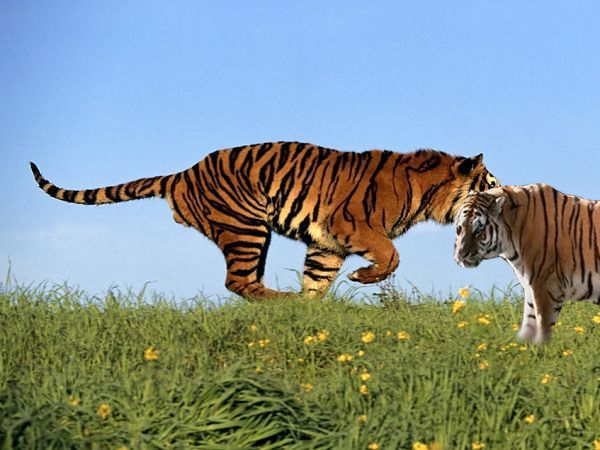
\includegraphics[width=12cm]{Figures/tiger.jpg}
\caption{Input image}
\label{fig:lion}
\end{figure}


\begin{figure}[h!]
\centering
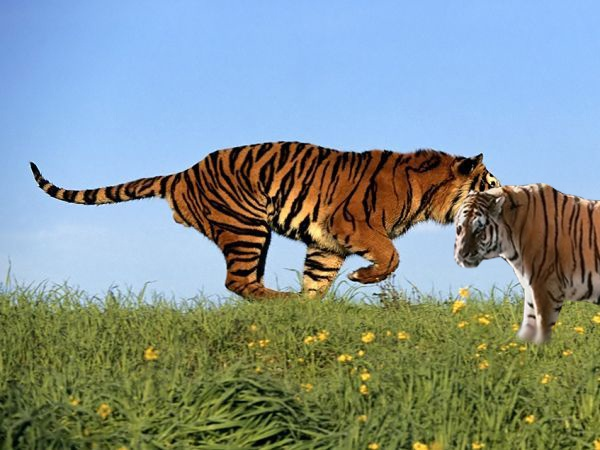
\includegraphics[width=12cm]{Figures/tiger_resaved.jpg}
\caption{Resaved image}
\label{fig:lion}
\end{figure}
With JPEG, saving a picture causes the colors to change a little as shown in fig 4.2

\begin{figure}[h!]
\centering
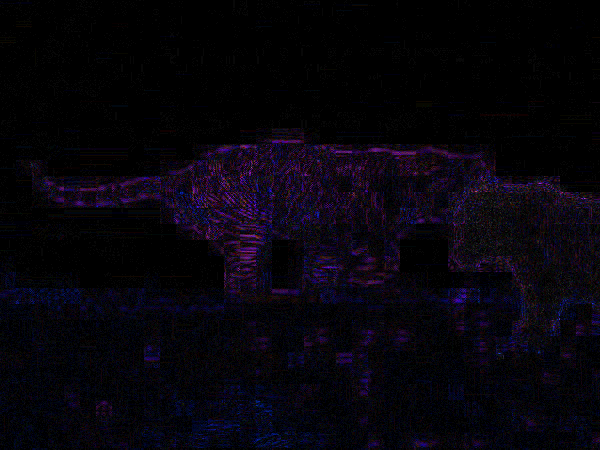
\includegraphics[width=12cm]{Figures/tiger_ela.png}
\caption{ELA image}
\label{fig:lion}
\end{figure}

\newpage
The ELA results highlight the areas in the image that are most prone to color degradation during a resave. This is shown in fig 4.3

\begin{figure}[h!]
\centering
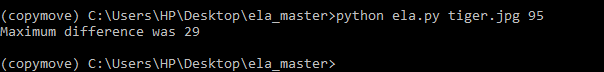
\includegraphics[width=16cm]{Figures/ela-cmd.PNG}
\caption{Error}
\label{fig:lion}
\end{figure}
The maximum difference which shows the error potential level when implemented is shown in fig 4.4

\newpage

\subsection{TRAINING THE CNN}
The output for this module is given below:

\begin{figure}[htp]
\centering
\includegraphics[width=13cm,height=7cm]{train2.PNG}
\caption{Training phase 1 }
\label{fig:lion}
\end{figure}
\begin{figure}[htp]
\centering
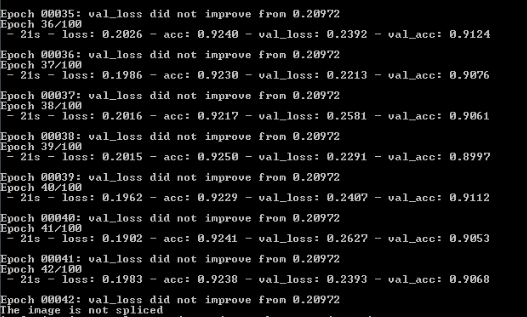
\includegraphics[width=13cm,height=7cm]{train1.PNG}
\caption{Training phase 2}
\label{fig:lion}
\end{figure}
 
The system is trained for 100 epochs with patience of 10 monitored upon the validation loss. Each time the system is trained the number of epochs varies depending on the change in the validation loss.

\subsection{FORGERY DETECTOR}
Identifying the image by  computing whether the image is forged or not is given below:


\begin{figure}[htp]
\centering
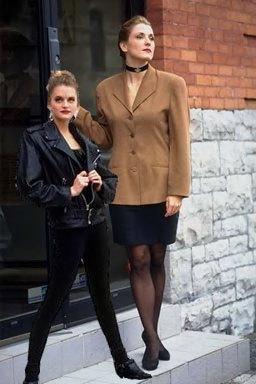
\includegraphics[width=8cm,height=8cm]{Figures/spli.jpg}
\caption{Type-Splicing }
\label{fig:lion}
\end{figure}

\begin{figure}[htp]
\centering
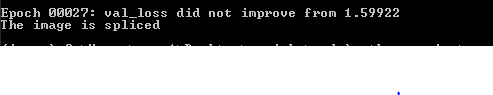
\includegraphics[width=15cm,height=4cm]{splicecmd.png}
\caption{Type-Splicing detection}
\label{fig:lion}
\end{figure}

The above image is identified to be a forged image undergone splicing. Hence it will not be further checked for copy move forgery.
\newpage
\begin{figure}[htp]
\centering
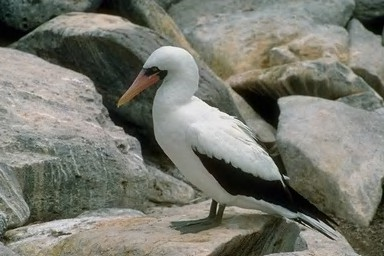
\includegraphics[width=10cm]{Figures/authen.jpg}
\caption{Authentic input}
\label{fig:lion}
\end{figure}


\begin{figure}[htp]
\centering
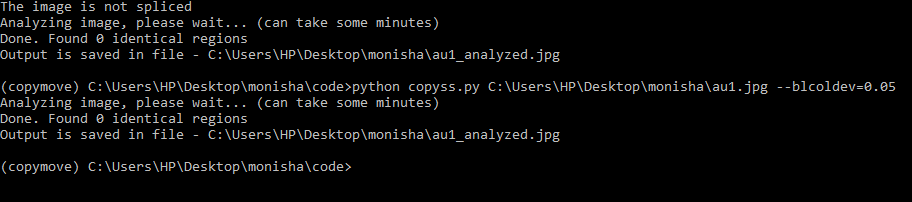
\includegraphics[width=15cm,height=5cm]{auth.PNG}
\caption{Authenticity detection}
\label{fig:lion}
\end{figure}
The above image is identified to be a not spliced image. Hence it will be further checked for copy move forgery. Since the image given is an authentic image which has not undergone any type of forgery no identical regions are found.
\newpage
\subsection{COPY MOVE TYPE DETECTION}
The output for this module is given below:


\begin{figure}[htp]
\centering
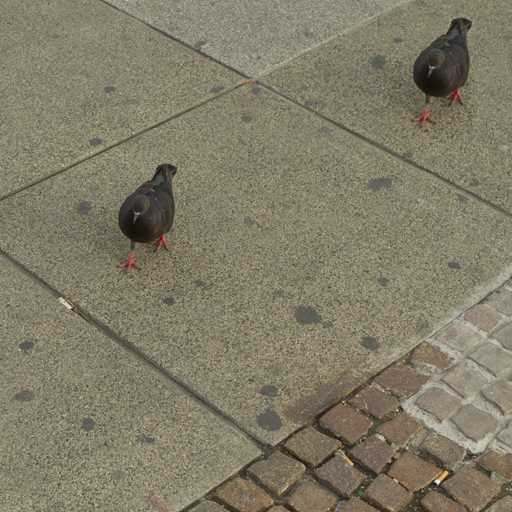
\includegraphics[width=7cm,height=5cm]{Figures/cmf.jpg}
\caption{Input image}
\label{fig:lion}
\end{figure}

\begin{figure}[htp]
\centering
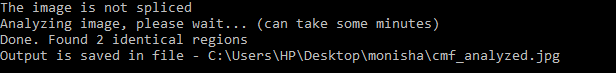
\includegraphics[width=14cm]{Figures/12.PNG}
\caption{Copy move detection}
\label{fig:lion}
\end{figure}

 
\begin{figure}[htp]
\centering
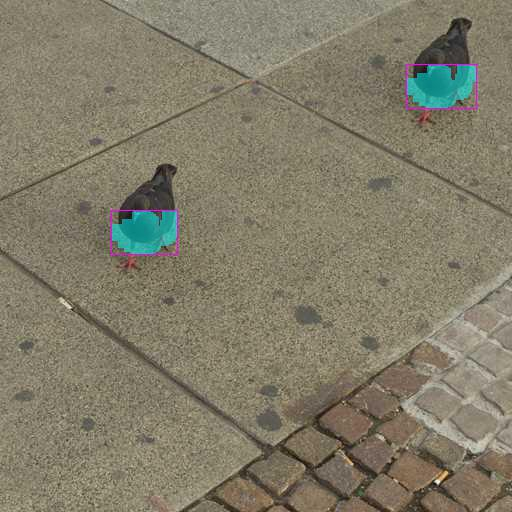
\includegraphics[width=7cm,height=5cm]{Figures/cmf_analyzed.jpg}
\caption{Output image}
\label{fig:lion}
\end{figure}
The above image is checked for splicing forgery and is detected to be not spliced. Hence it will be further checked for copy move forgery and is identified to have undergone the same.

\newpage
\section{PERFORMANCE METRICS}
The different  metrices  are  used  to  evaluate  the classification algorithm,  such  as confusion  matrices  for Precision,  Recall,  F-measure,  and  Accuracy.  
\subsubsection{Precision}

Proportion of predicted positives which are actual positive

         \newline
          Precision  = TP / (TP + FP)
\subsubsection{Recall}

\tab Proportion of actual positives which are predicted positive
        
         \newline
          Recall  = TP / (TP + FN)

\subsubsection{F-measure}

This is evaluated by the harmonic mean between precision, recall.

        \newline
         F-measure =    2 ∗ ((precision * recall)/(precision + recall))
\subsubsection{Accuracy}

\tab This is calculated as the proportion of true positive,true negatives and true results from all the given data. 

        \newline
        Accuracy  = (TP + TN) / (TP + TN + FP + FN)
\subsubsection{Error rate}
        Error Rate= 1  -  Accuracy. 
        
\newpage
\begin{figure}[htp]
\centering
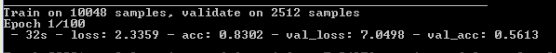
\includegraphics[width=14cm]{Figures/sample.PNG}
\caption{No of samples used for training and testing}
\label{fig:lion}
\end{figure}       
The model is trained with 80\% of the total samples which is about 10048 images of 12560 images in the dataset and tested with the rest 20\% data which is 2512 images.

\begin{figure}[htp]
\centering
\includegraphics[width=14cm]{Figures/train2.PNG}
\caption{Validation accuracy calculated at each epoch}
\label{fig:lion}
\end{figure}
\newpage
\bigskip
\begin{figure}[htp]
\centering
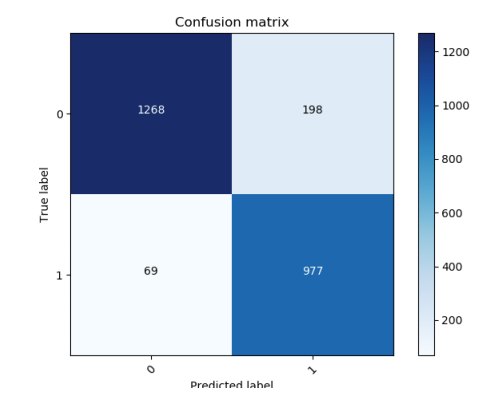
\includegraphics[width=15cm,height=10cm]{Figures/matrix.PNG}
\caption{Confusion matrix of results of CNN on testdata}
\label{fig:lion}
\end{figure}

The validation accuracy at final epochs is maintained to 90.68 percentage.

